\section{Interfaces}

En esta sección se documentan las distintas interfaces gráficas y conversacionales que componen el ecosistema de \textbf{SocioUnido}, abarcando las soluciones para socios, empleados, personal administrativo y sistemas de control.

Como SocioUnido es una plataforma de \textbf{marca blanca}, los ejemplos a continuación muestran dos escenarios (la versión base/neutra y una versión adaptada). Para ilustrar la adaptabilidad del sistema sin generar rivalidades ni preferencias en el contexto del fútbol argentino, se ha seleccionado al club \textbf{Mamelodi Sundowns} de Sudáfrica como caso de uso. Esto permite demostrar una interfaz 100\% funcional y personalizada manteniendo la neutralidad institucional del proyecto.

\subsection{HealthChecker}

Panel de control dedicado al monitoreo continuo de la infraestructura. Esta interfaz permite al equipo técnico visualizar en tiempo real el estado y la disponibilidad del ecosistema.

\begin{figure}[h!]
    \centering
    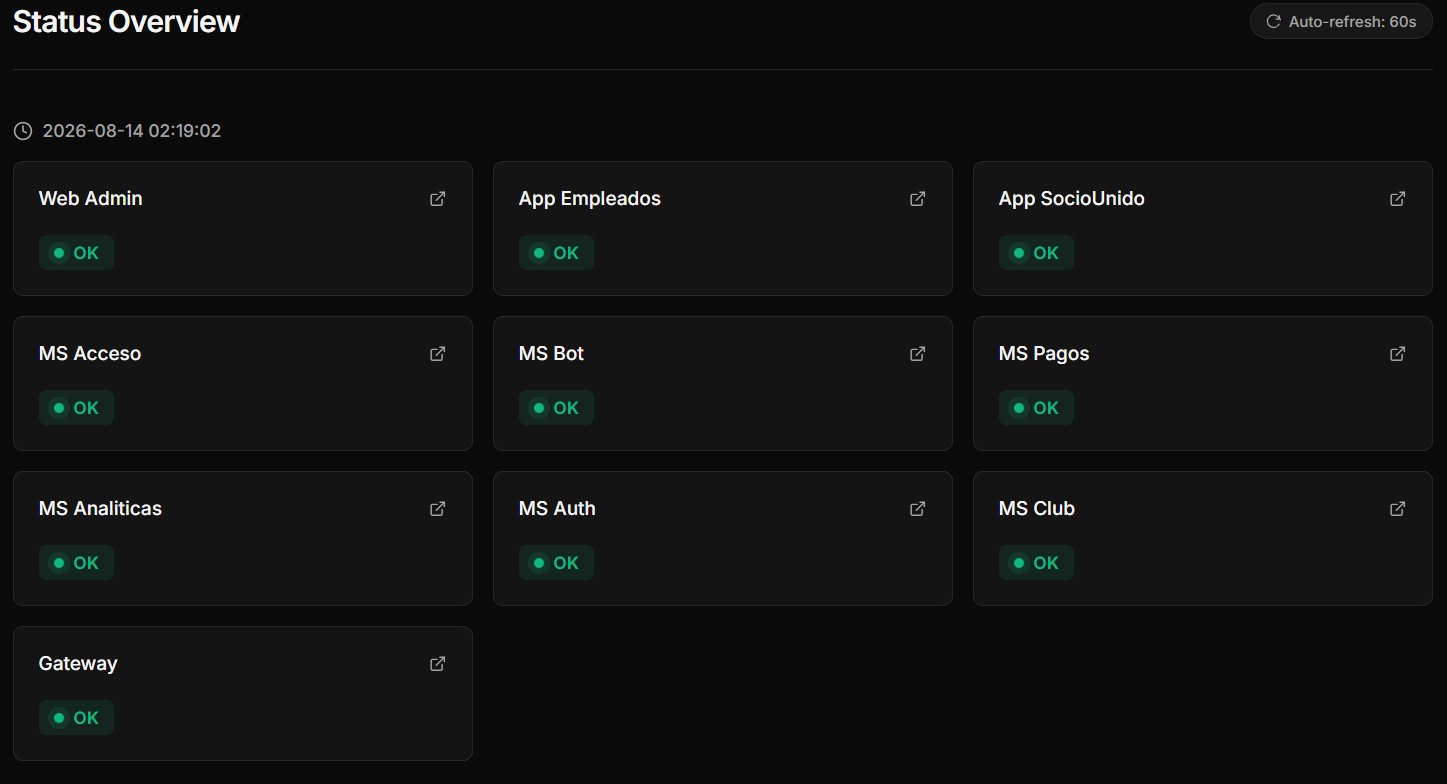
\includegraphics[width=0.9\textwidth]{img/healthchecker/healthchecker.png}
    \caption{Vista del Healthchecker. Estado actual de las instancias y servicios desplegados.}
    \label{fig:ui_healthchecker}
\end{figure}

\newpage

\subsection{Plataforma web (Panel de gestión)}

La plataforma web es el panel administrativo centralizado orientado a la dirigencia, administración y personal operativo del club. Permite la gestión integral del padrón, métricas financieras, disciplinas y configuración de la tienda.

\subsubsection{Login y autenticación}
\begin{figure}[h!]
    \centering
    \textbf{Marca blanca (neutro)} \\ \vspace{0.2cm}
    
\includegraphics[width=0.9\textwidth]{img/plataforma-web/login-neutro.jpeg} \\
    \vspace{0.8cm}
    \textbf{Mamelodi Sundowns} \\ \vspace{0.2cm}
    
\includegraphics[width=0.9\textwidth]{img/plataforma-web/login-mamelodi.jpeg}
    \caption{Comparativa de vistas: Login y autenticación.}
\end{figure}

\newpage

\subsubsection{Inicio (Home)}
\begin{figure}[h!]
    \centering
    \textbf{Marca blanca (neutro)} \\ \vspace{0.2cm}
    
\includegraphics[width=\textwidth]{img/plataforma-web/home-neutro.jpeg} \\
    \vspace{0.8cm}
    \textbf{Mamelodi Sundowns} \\ \vspace{0.2cm}
    
\includegraphics[width=\textwidth]{img/plataforma-web/home-mamelodi.jpeg}
    \caption{Comparativa de vistas: Panel principal (Home).}
\end{figure}

\newpage

\subsubsection{Métricas y estadísticas}
\begin{figure}[h!]
    \centering
    \textbf{Marca blanca (neutro)} \\ \vspace{0.2cm}
    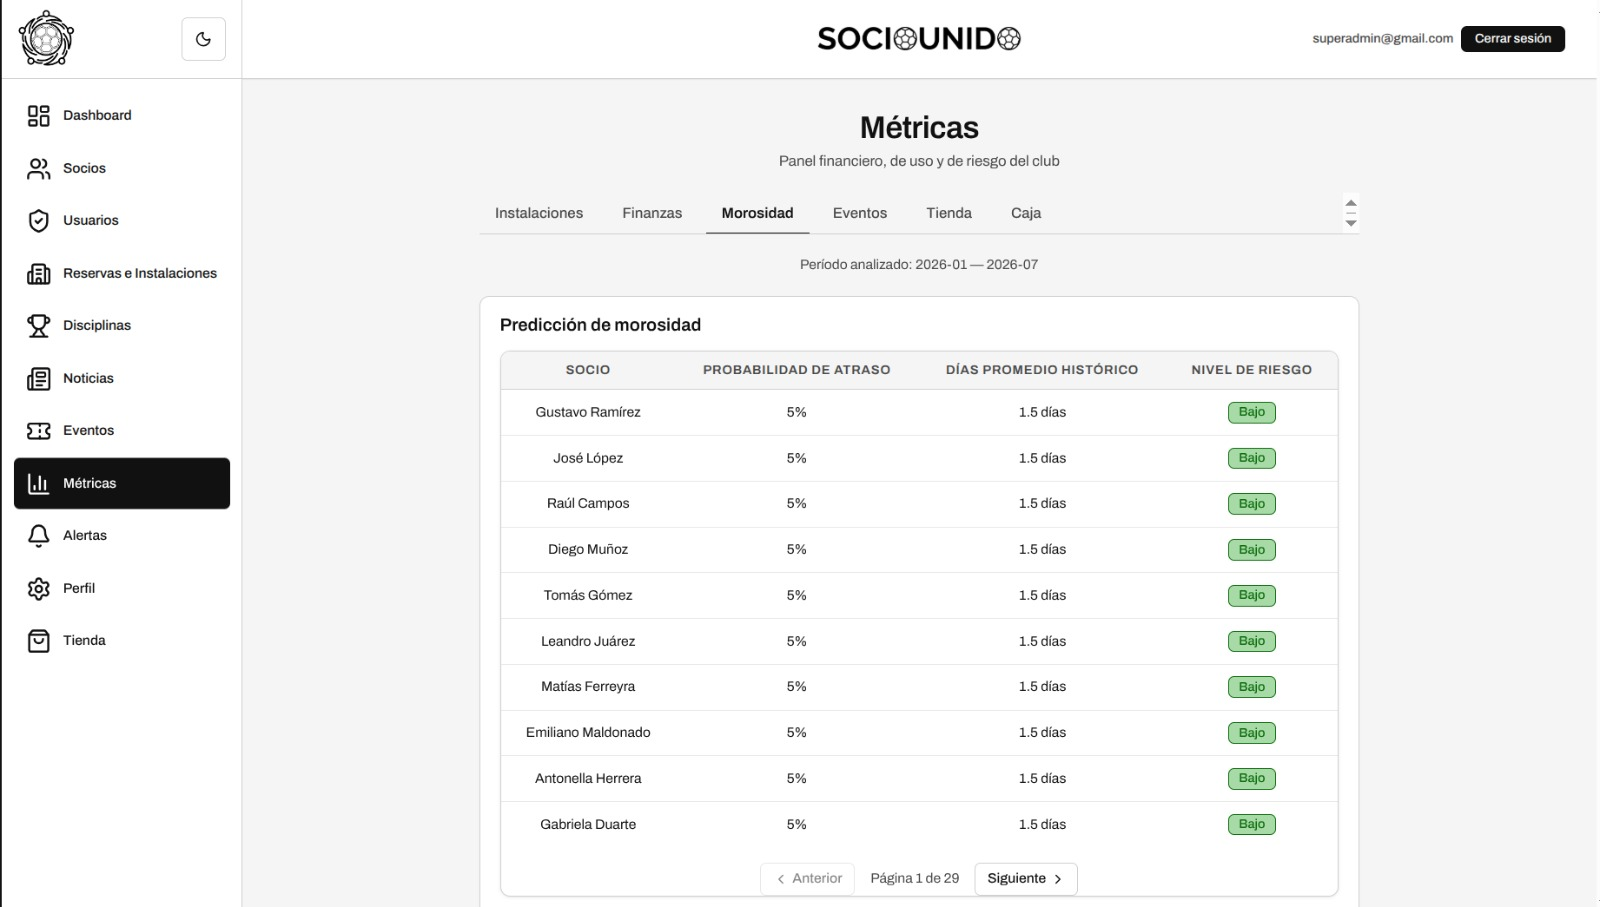
\includegraphics[width=\textwidth]{img/plataforma-web/metricas-neutro.jpeg} \\
    \vspace{0.8cm}
    \textbf{Mamelodi Sundowns} \\ \vspace{0.2cm}
    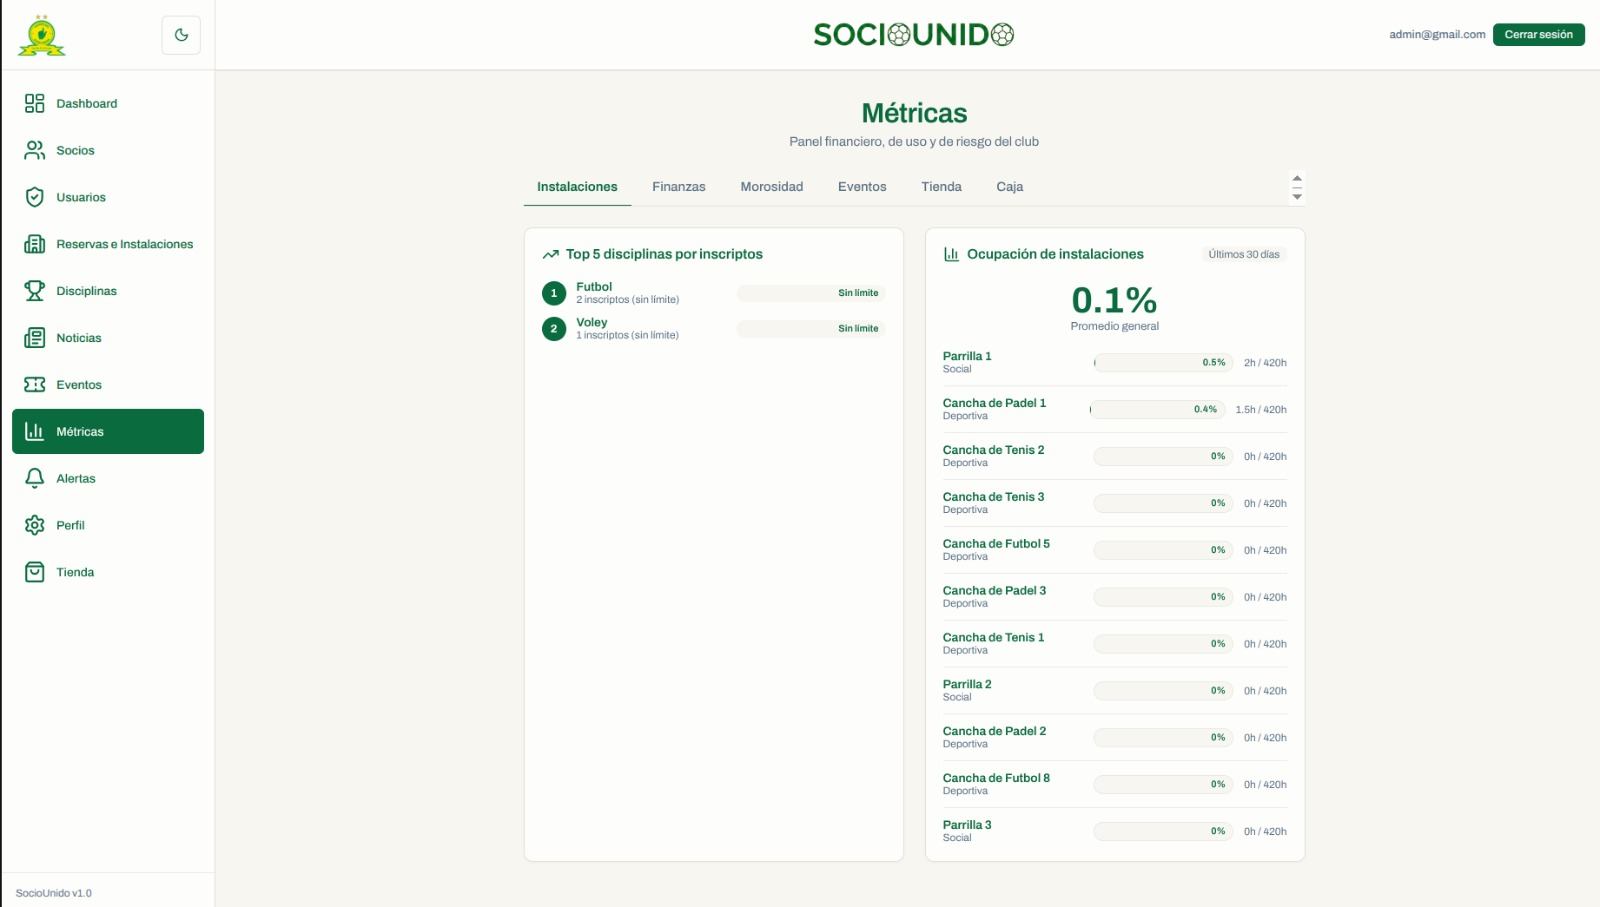
\includegraphics[width=\textwidth]{img/plataforma-web/metricas-mamelodi.jpeg}
    \caption{Comparativa de vistas: Panel de métricas y estadísticas.}
\end{figure}

\newpage

\subsubsection{Gestión de socios y perfil específico}
\begin{figure}[h!]
    \centering
    \textbf{Padrón general (Mamelodi Sundowns)} \\ \vspace{0.2cm}
    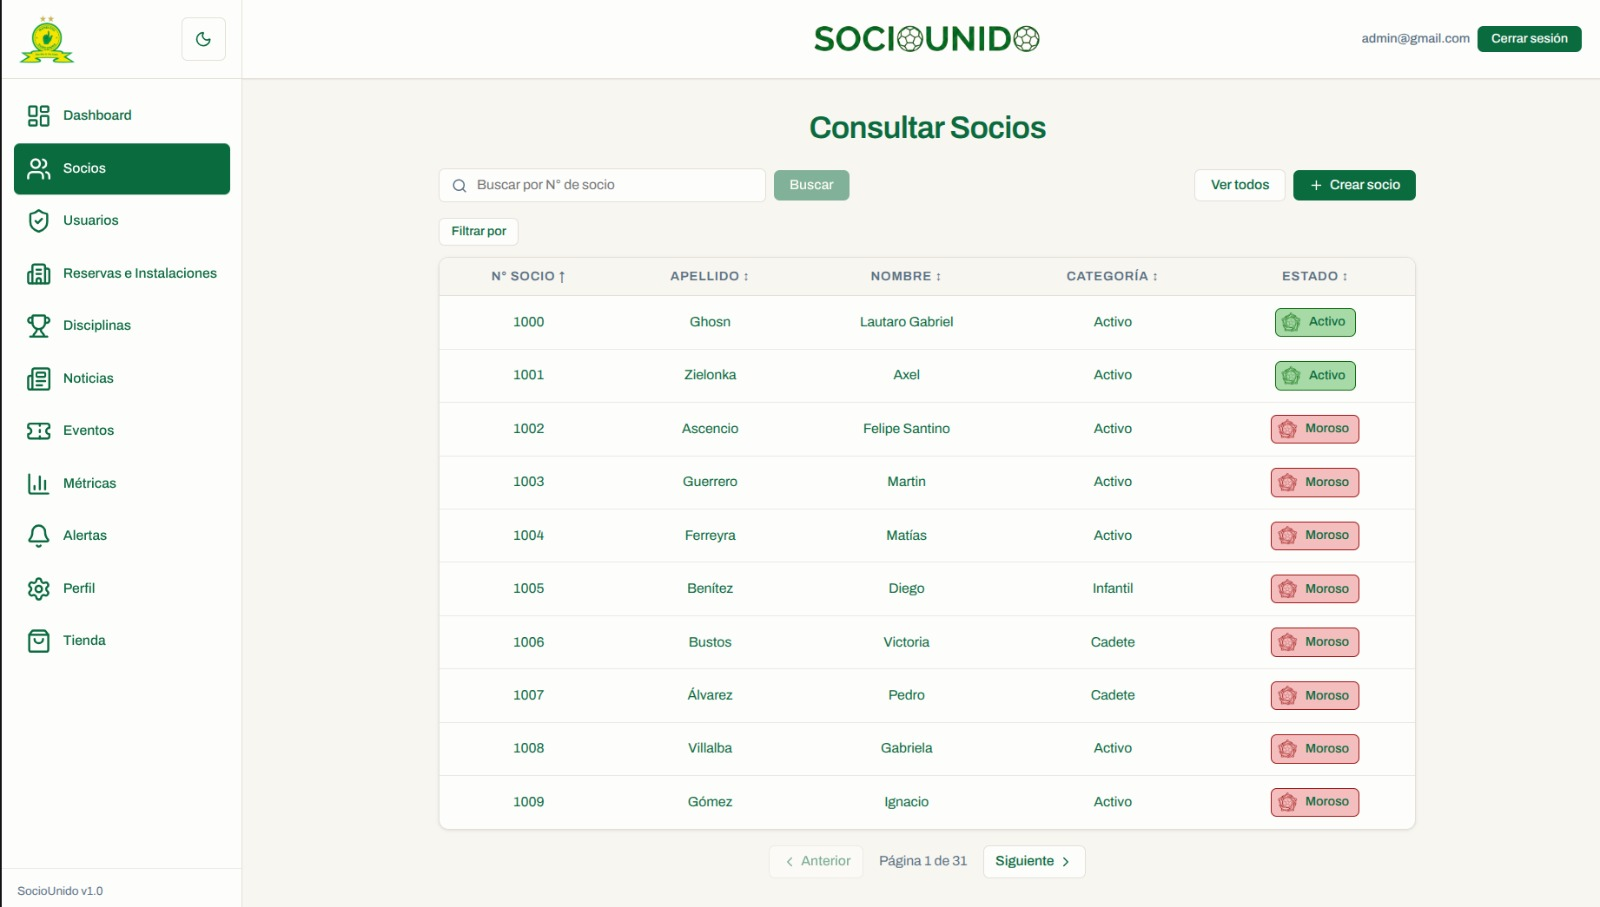
\includegraphics[width=\textwidth]{img/plataforma-web/socios-mamelodi.jpeg} \\
    \vspace{0.8cm}
    \textbf{Perfil de socio (Mamelodi Sundowns)} \\ \vspace{0.2cm}
    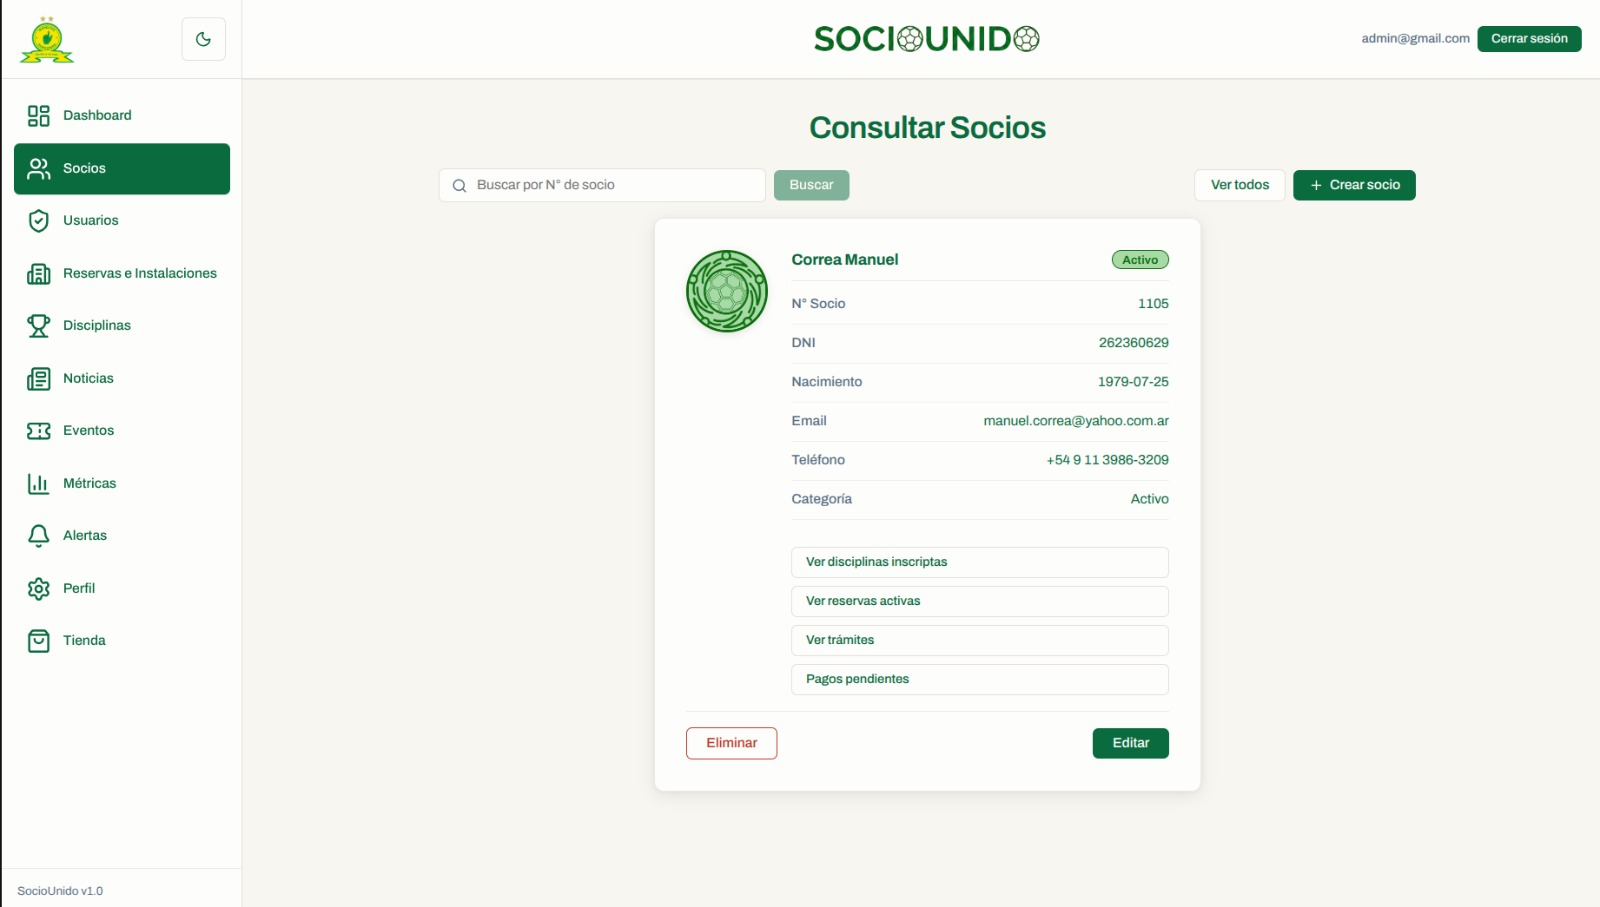
\includegraphics[width=\textwidth]{img/plataforma-web/socio-especifico-mamelodi.jpeg}
    \caption{Vistas de gestión societaria implementadas para el club de ejemplo.}
\end{figure}

\newpage

\subsubsection{Gestión de disciplinas y tienda}
\begin{figure}[h!]
    \centering
    \textbf{Disciplinas general (Mamelodi Sundowns)} \\ \vspace{0.2cm}
    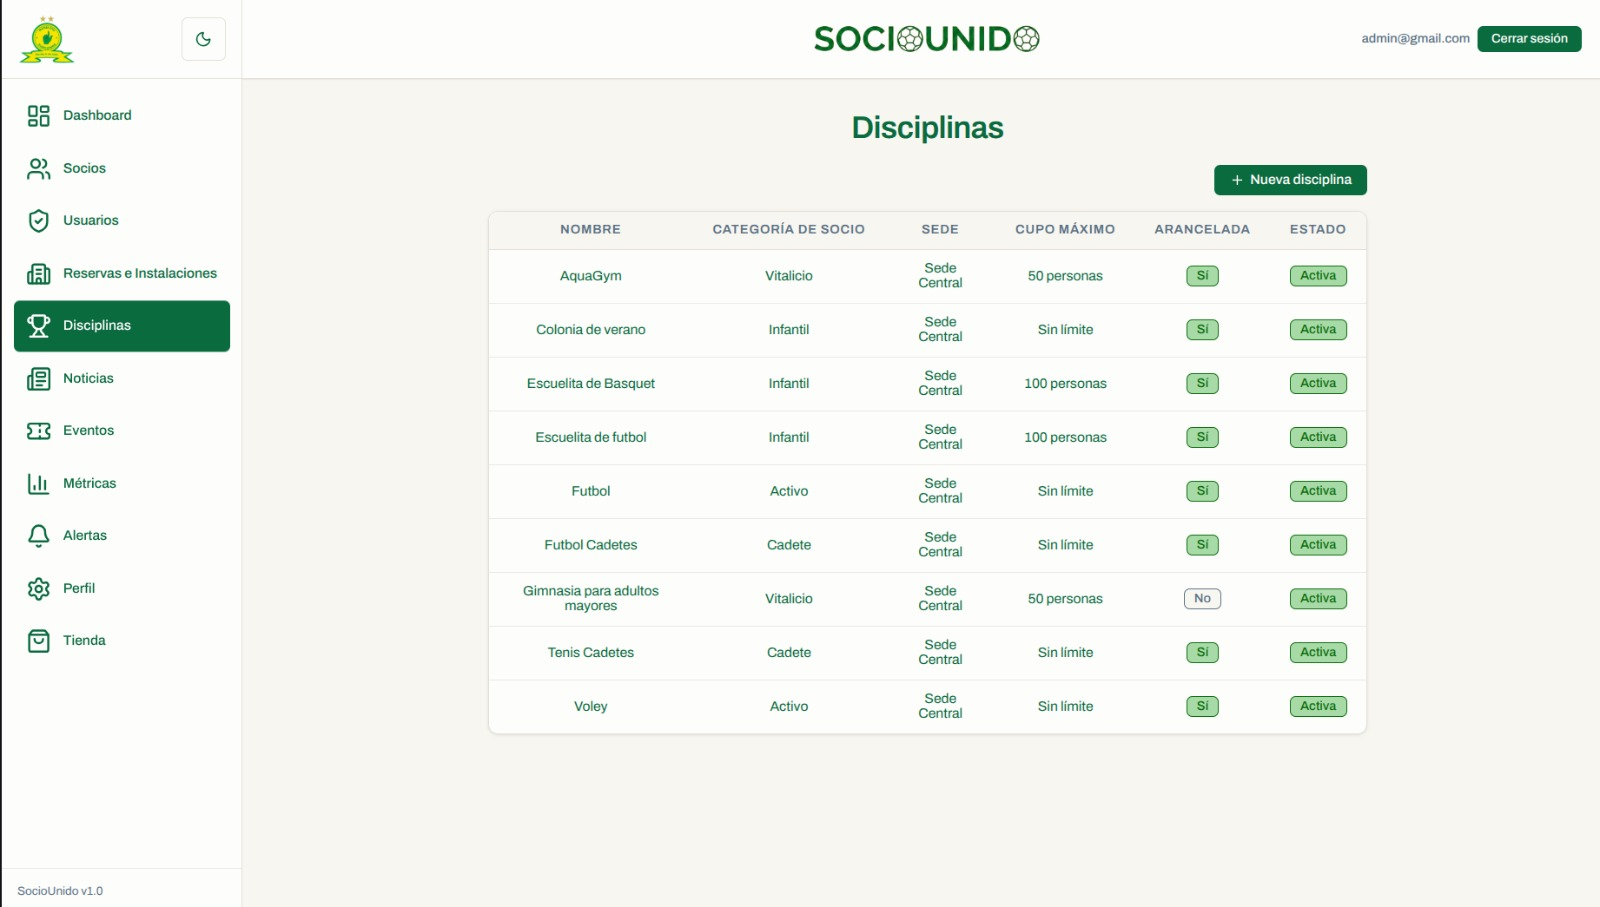
\includegraphics[width=\textwidth]{img/plataforma-web/disciplinas-mamelodi.jpeg} \\
    \vspace{0.8cm}
    \textbf{Tienda institucional (Mamelodi Sundowns)} \\ \vspace{0.2cm}
    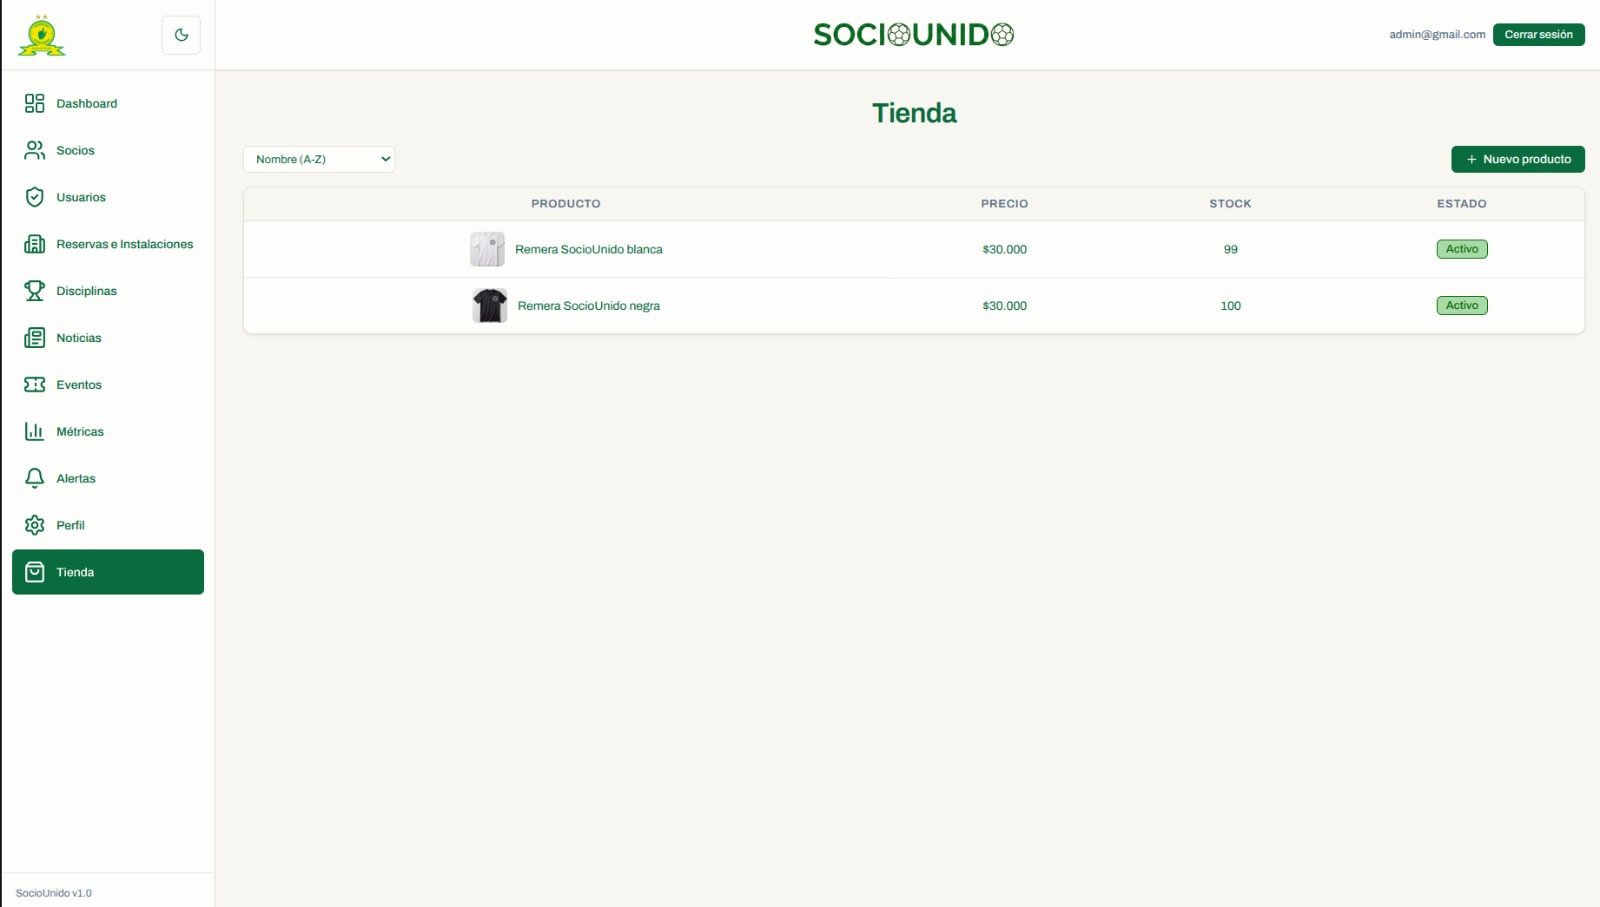
\includegraphics[width=\textwidth]{img/plataforma-web/tienda-mamelodi.jpeg}
    \caption{Vistas de disciplinas y e-commerce implementadas para el club de ejemplo.}
\end{figure}

\newpage

\subsection{App del socio (PWA)}

Aplicación Web Progresiva diseñada para el usuario final. Centraliza la experiencia del asociado permitiéndole gestionar su perfil, abonar cuotas, y acceder a su carnet digital de manera ágil y con soporte offline.

\subsubsection{Pantalla de acceso (Login)}
\begin{figure}[h!]
    \centering
    \begin{minipage}{0.45\textwidth}
        \centering
        \textbf{Marca blanca (neutro)} \\ \vspace{0.2cm}
        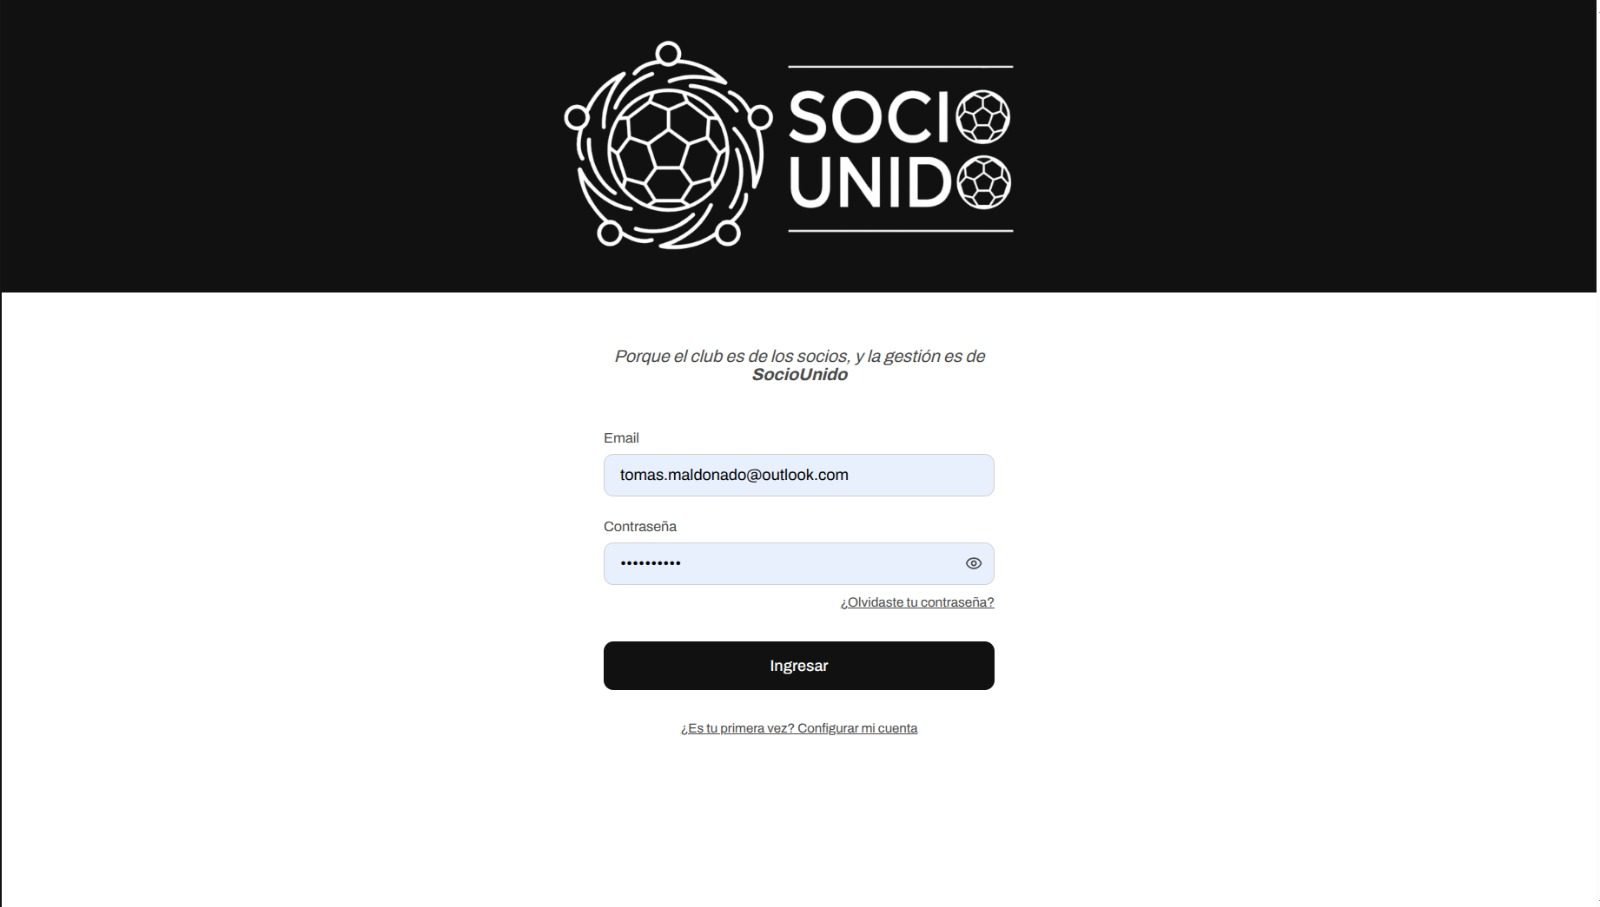
\includegraphics[width=\textwidth]{img/app-socio/login-neutro.jpeg}
    \end{minipage}\hfill
    \begin{minipage}{0.45\textwidth}
        \centering
        \textbf{Mamelodi Sundowns} \\ \vspace{0.2cm}
        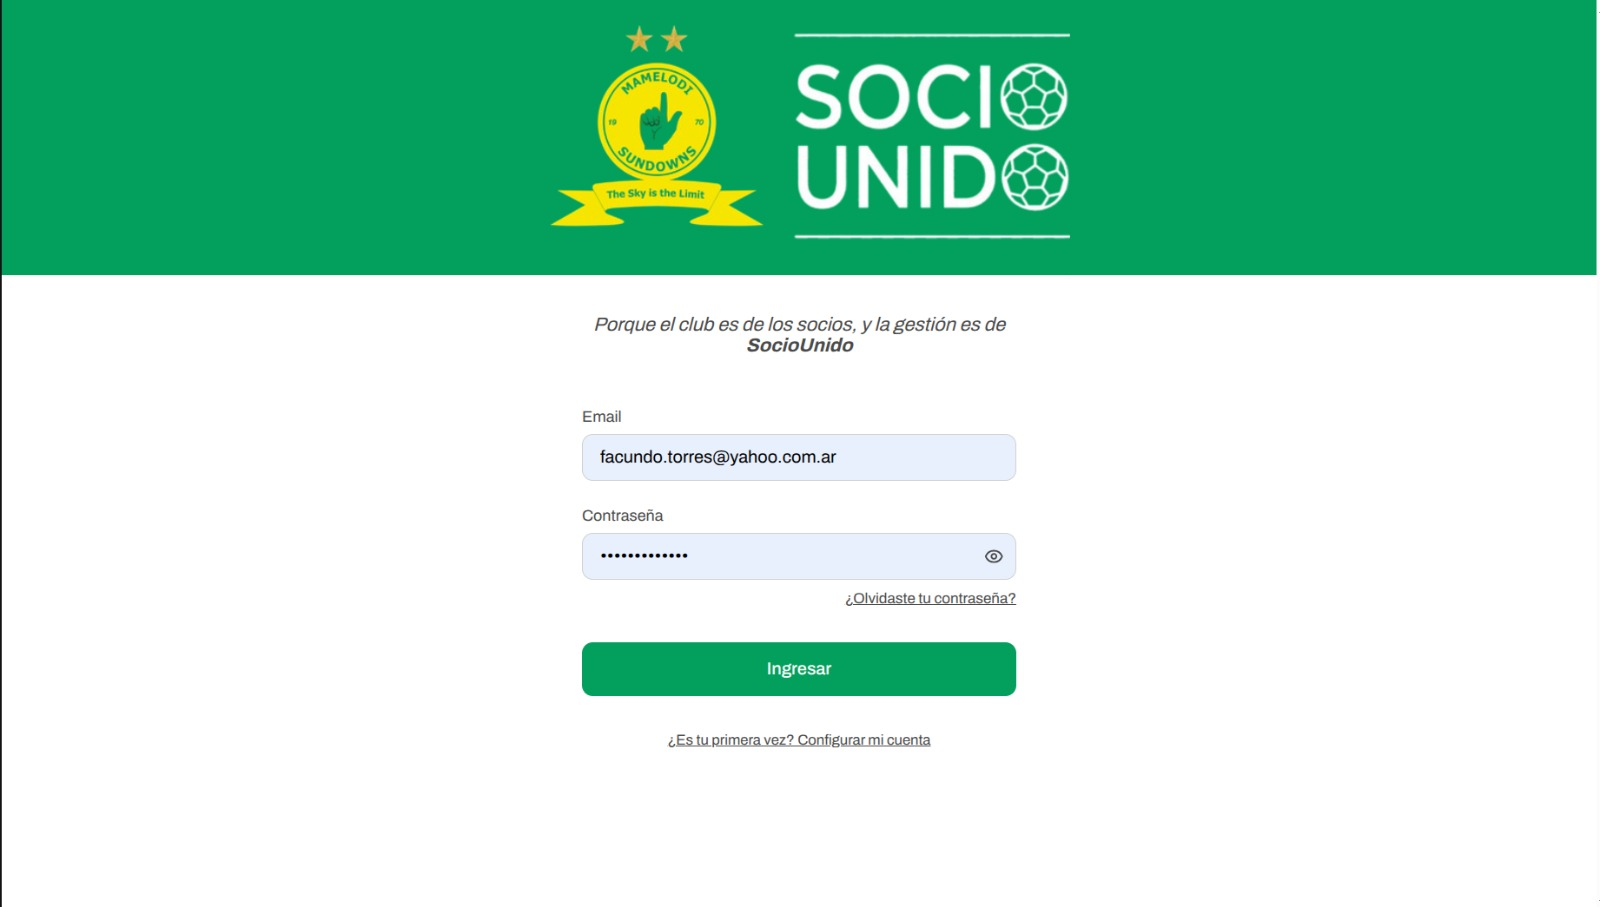
\includegraphics[width=\textwidth]{img/app-socio/login-mamelodi.jpeg}
    \end{minipage}
    \caption{Comparativa: Pantalla de acceso - App del socio.}
\end{figure}

\subsubsection{Inicio (Dashboard del socio)}
\begin{figure}[h!]
    \centering
    \begin{minipage}{0.45\textwidth}
        \centering
        \textbf{Marca blanca (neutro)} \\ \vspace{0.2cm}
        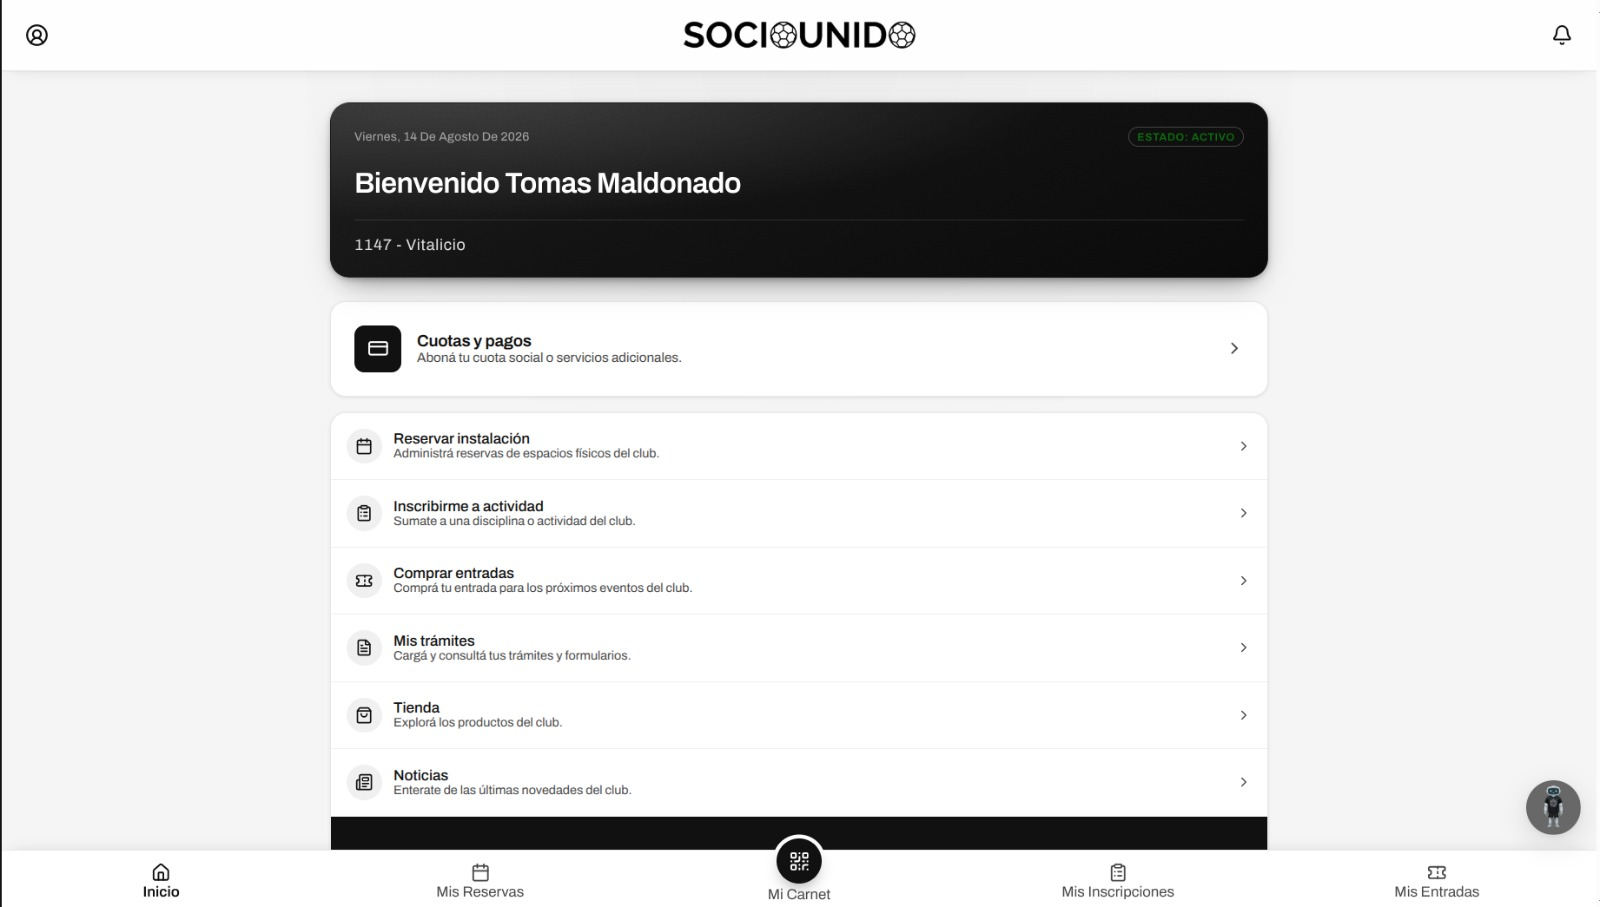
\includegraphics[width=\textwidth]{img/app-socio/home-neutro.jpeg}
    \end{minipage}\hfill
    \begin{minipage}{0.45\textwidth}
        \centering
        \textbf{Mamelodi Sundowns} \\ \vspace{0.2cm}
        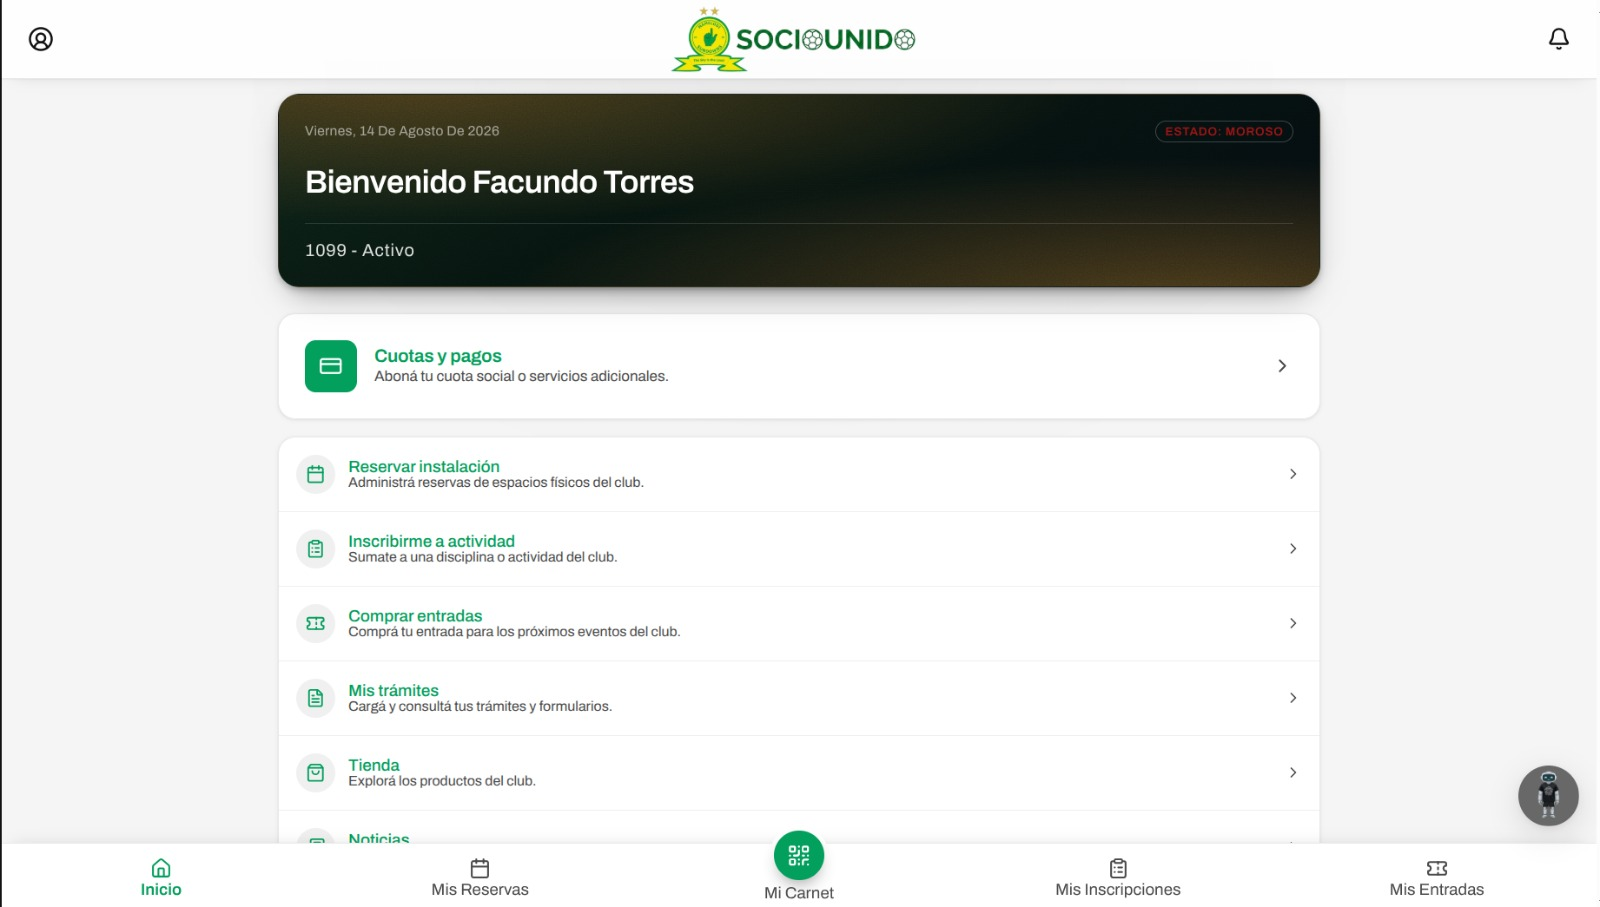
\includegraphics[width=\textwidth]{img/app-socio/home-mamelodi.jpeg}
    \end{minipage}
    \caption{Comparativa: Inicio - App del socio.}
\end{figure}

\newpage

\subsubsection{Perfil de usuario y pagos}
\begin{figure}[h!]
    \centering
    \begin{minipage}{0.45\textwidth}
        \centering
        \textbf{Perfil (Mamelodi Sundowns)} \\ \vspace{0.2cm}
        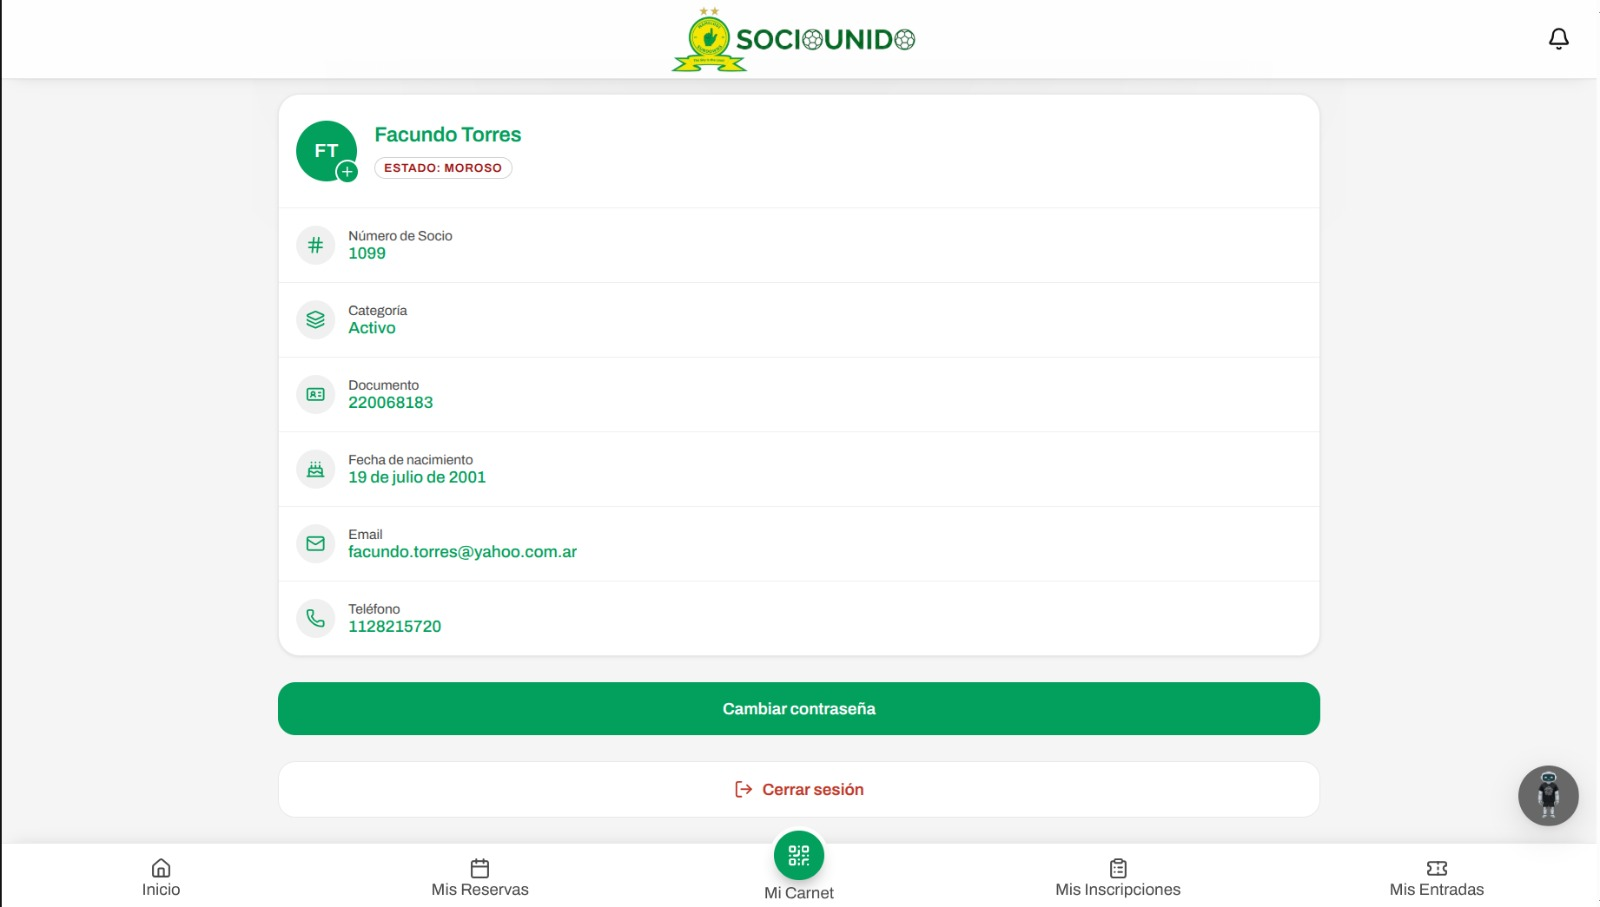
\includegraphics[width=\textwidth]{img/app-socio/perfil-mamelodi.jpeg}
    \end{minipage}\hfill
    \begin{minipage}{0.45\textwidth}
        \centering
        \textbf{Pagos (Mamelodi Sundowns)} \\ \vspace{0.2cm}
        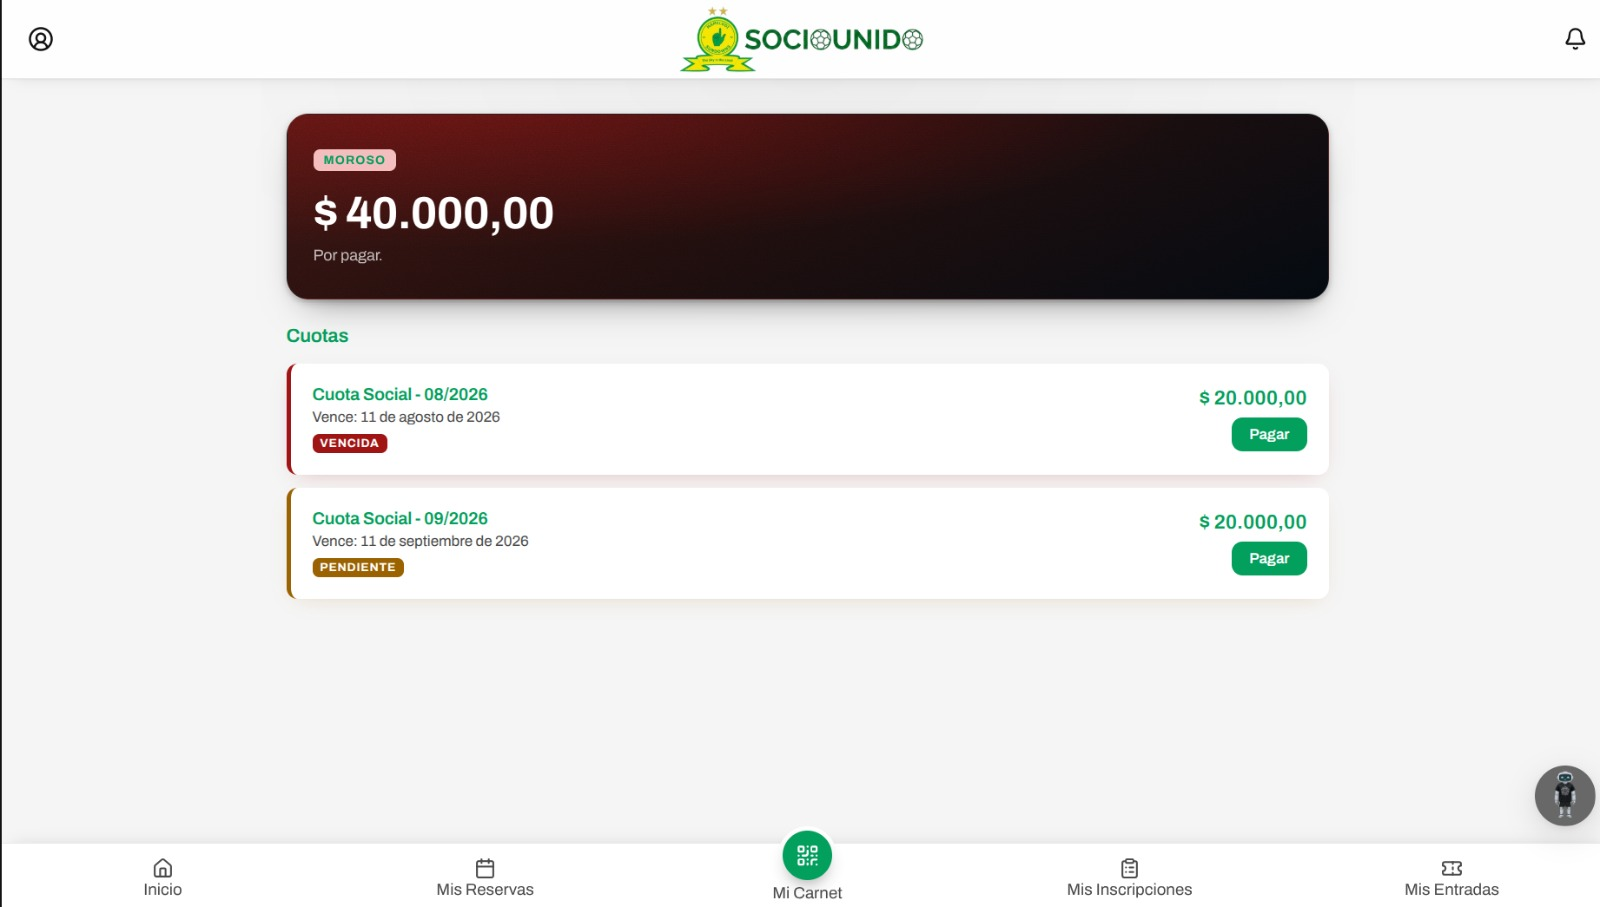
\includegraphics[width=\textwidth]{img/app-socio/pagos-mamelodi.jpeg}
    \end{minipage}
    \caption{Vistas de perfil y estado de pagos - App del socio.}
\end{figure}

\subsubsection{Carnet digital (Acceso inteligente)}
\begin{figure}[h!]
    \centering
    \begin{minipage}{0.45\textwidth}
        \centering
        \textbf{Marca blanca (neutro)} \\ \vspace{0.2cm}
        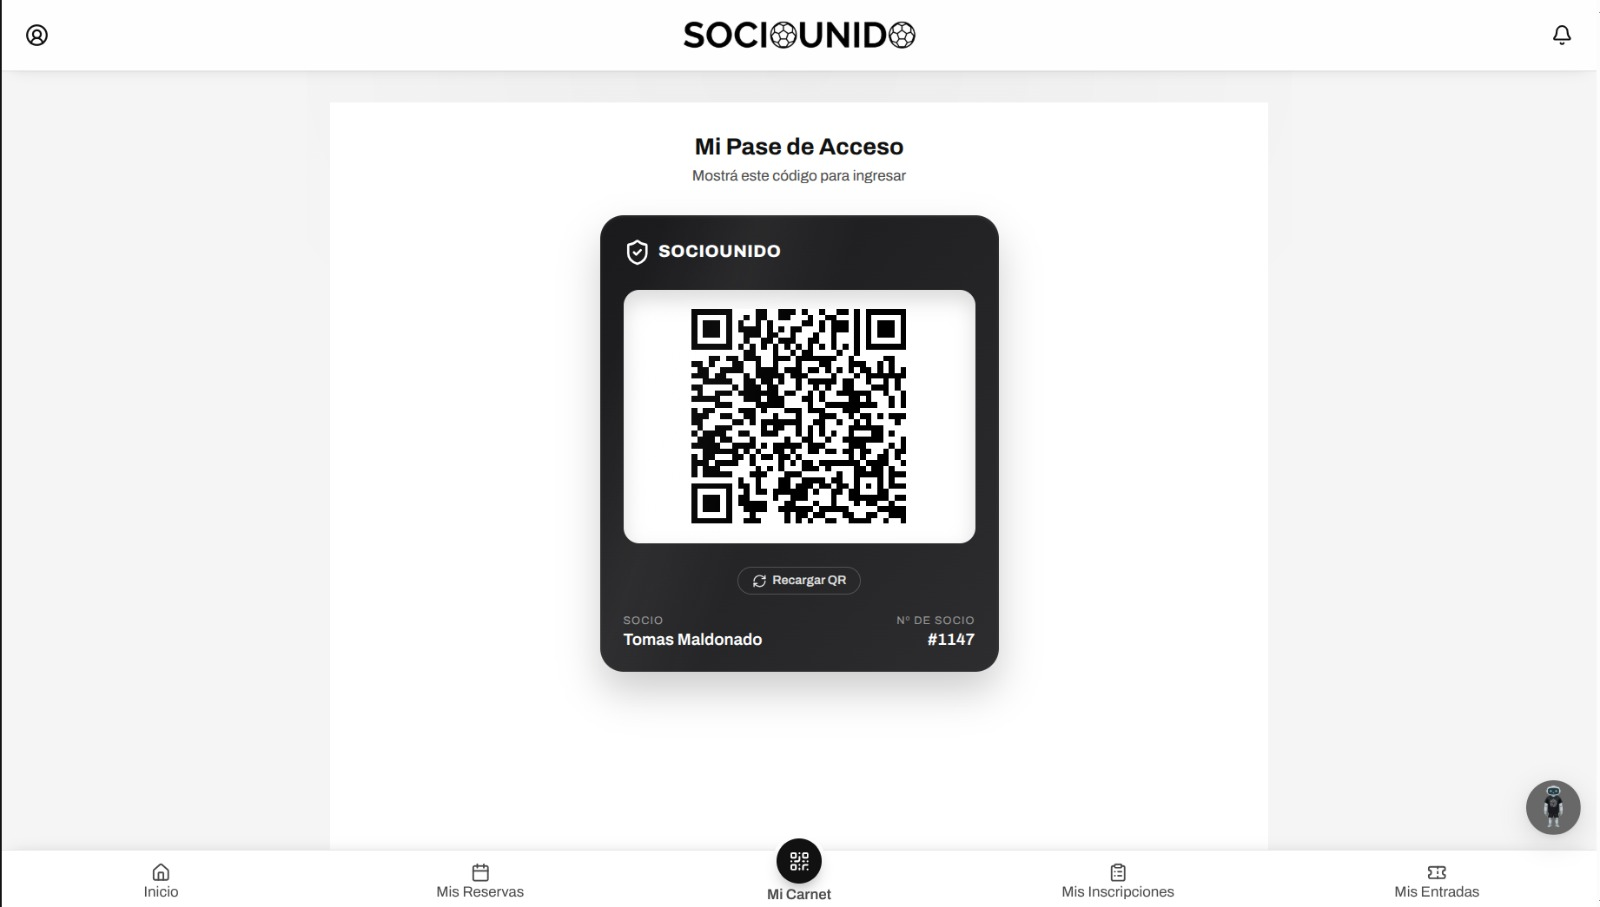
\includegraphics[width=\textwidth]{img/app-socio/carnet-neutro.jpeg}
    \end{minipage}\hfill
    \begin{minipage}{0.45\textwidth}
        \centering
        \textbf{Mamelodi Sundowns} \\ \vspace{0.2cm}
        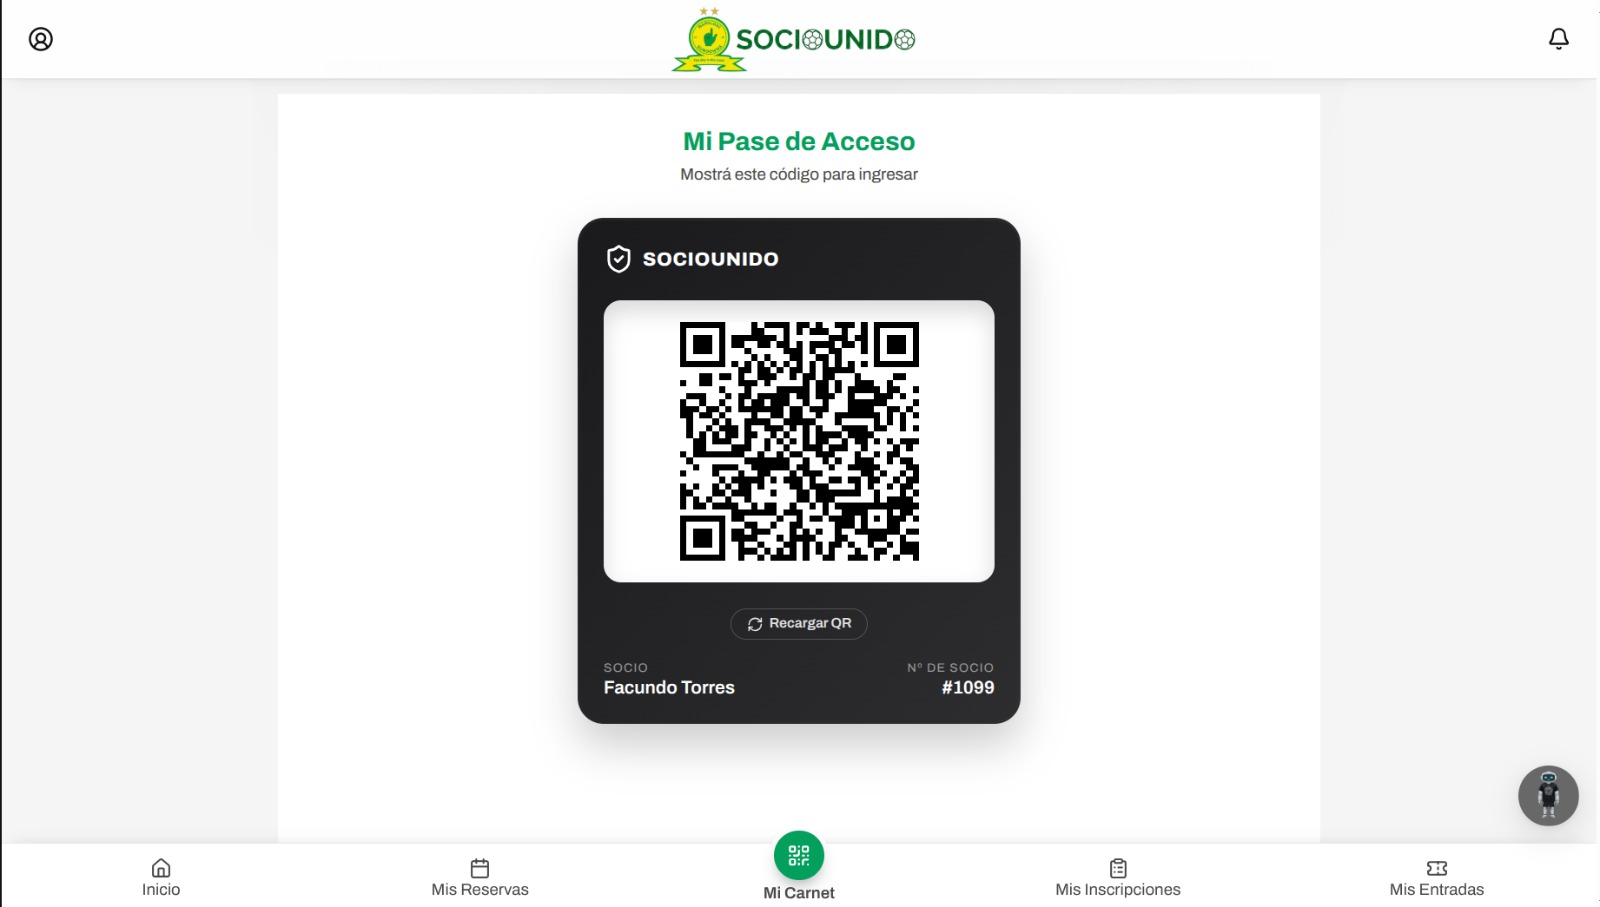
\includegraphics[width=\textwidth]{img/app-socio/carnet-mamelodi.jpeg}
    \end{minipage}
    \caption{Comparativa: Carnet digital - App del socio.}
\end{figure}

\newpage

\subsection{App del empleado (PWA)}

Aplicación móvil orientada al personal operativo y de campo del club. Está diseñada para facilitar las tareas cotidianas, la lectura rápida de credenciales y el control de accesos en los molinetes o puntos de entrada institucionales.

\subsubsection{Acceso y panel principal}
\begin{figure}[h!]
    \centering
    \begin{minipage}{0.45\textwidth}
        \centering
        \textbf{Login (Mamelodi Sundowns)} \\ \vspace{0.2cm}
        
\includegraphics[width=\textwidth]{img/app-trabajadores/login-mamelodi.jpeg}
    \end{minipage}\hfill
    \begin{minipage}{0.45\textwidth}
        \centering
        \textbf{Home (Mamelodi Sundowns)} \\ \vspace{0.2cm}
        
\includegraphics[width=\textwidth]{img/app-trabajadores/home-mamelodi.jpeg}
    \end{minipage}
    \caption{Vistas de acceso y panel principal operativo - App del empleado.}
\end{figure}

\subsubsection{Lector de código QR}
\begin{figure}[h!]
    \centering
    \begin{minipage}{0.45\textwidth}
        \centering
        \textbf{Marca blanca (neutro)} \\ \vspace{0.2cm}
        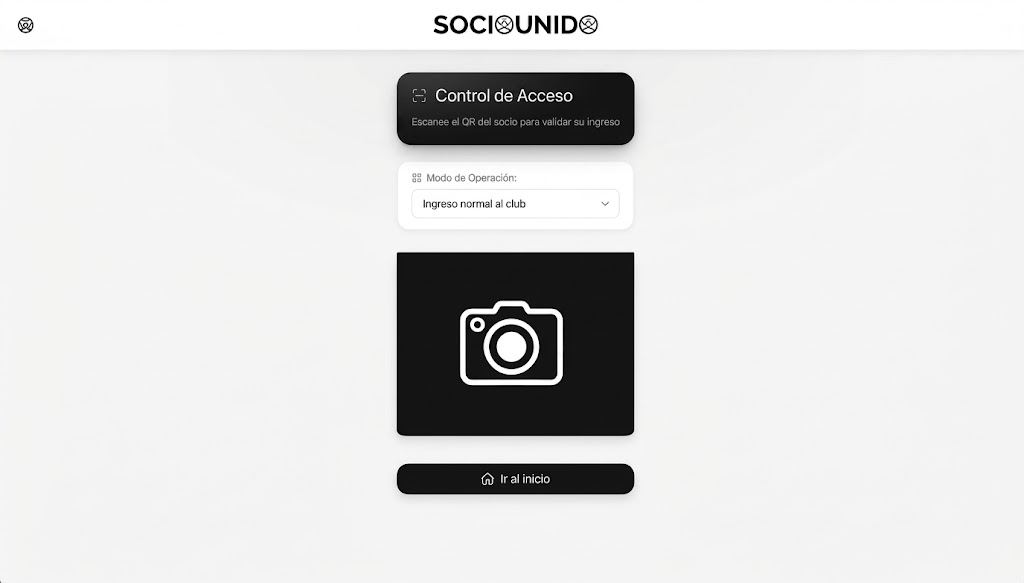
\includegraphics[width=\textwidth]{img/app-trabajadores/qr-neutro.jpg}
    \end{minipage}\hfill
    \begin{minipage}{0.45\textwidth}
        \centering
        \textbf{Mamelodi Sundowns} \\ \vspace{0.2cm}
        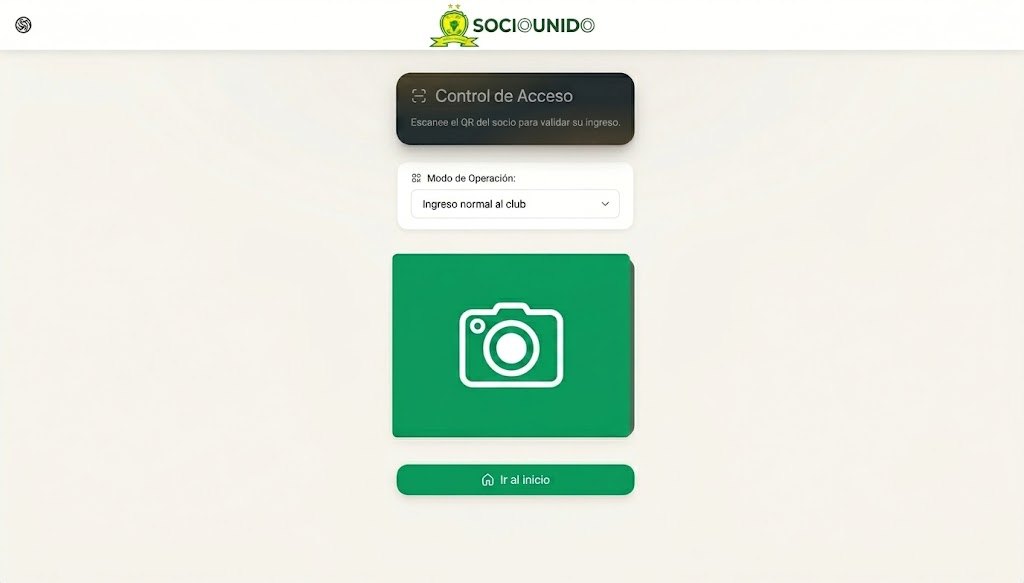
\includegraphics[width=\textwidth]{img/app-trabajadores/qr-mamelodi.jpg}
    \end{minipage}
    \caption{Comparativa: Lector de código QR - App del empleado.}
\end{figure}

\newpage

\subsection{Bot conversacional (BotIn)}

\textbf{BotIn} es el asistente virtual de la plataforma, integrado nativamente con Telegram a través del procesamiento de lenguaje natural (NLP). Facilita la autogestión de los socios respondiendo consultas frecuentes, asistiendo en el pago de cuotas y brindando soporte 24/7.

\begin{figure}[h!]
    \centering
    \begin{minipage}{0.45\textwidth}
        \centering
        \textbf{Perfil institucional} \\ \vspace{0.2cm}
        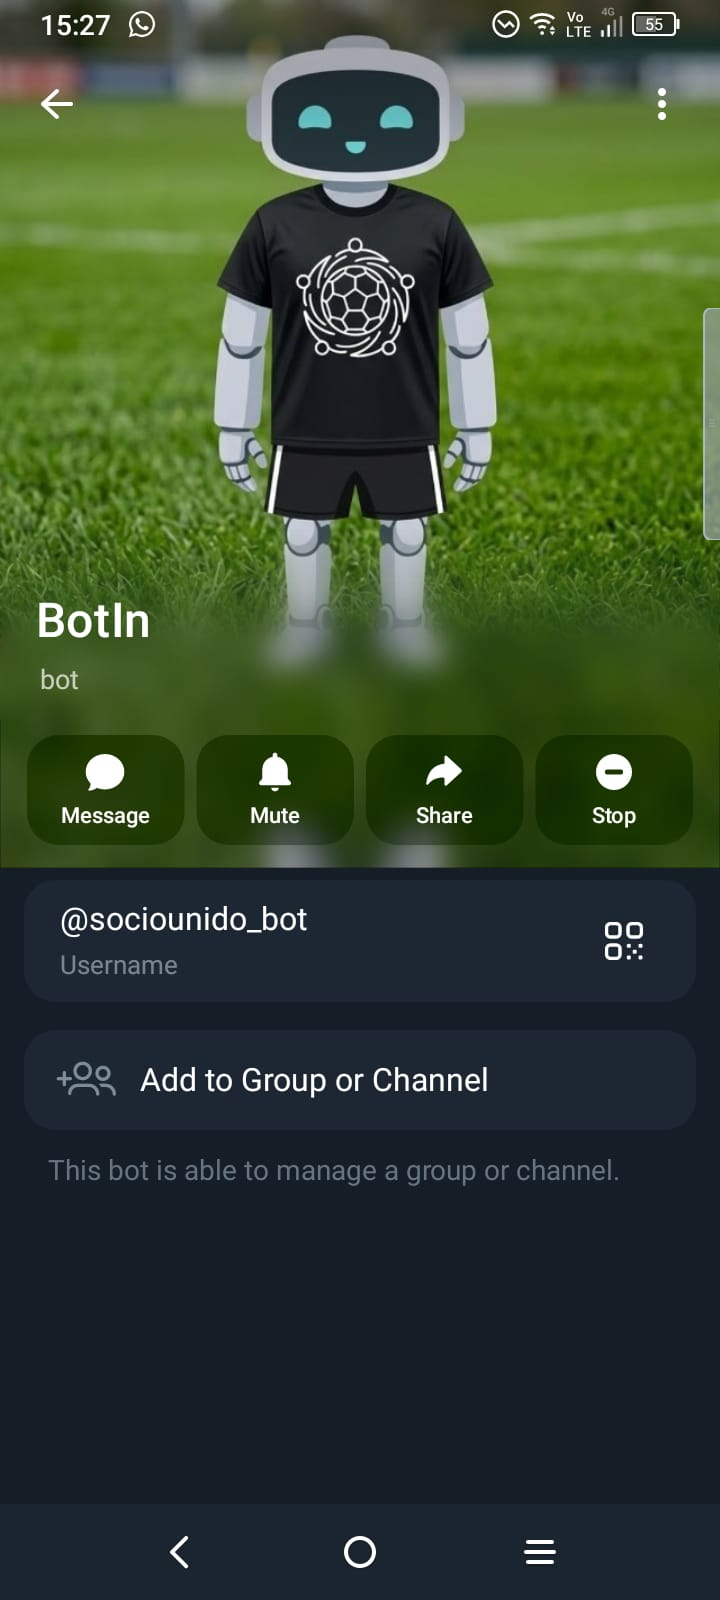
\includegraphics[width=\textwidth]{img/bot/perfil.jpeg}
    \end{minipage}\hfill
    \begin{minipage}{0.45\textwidth}
        \centering
        \textbf{Interacción (Chat)} \\ \vspace{0.2cm}
        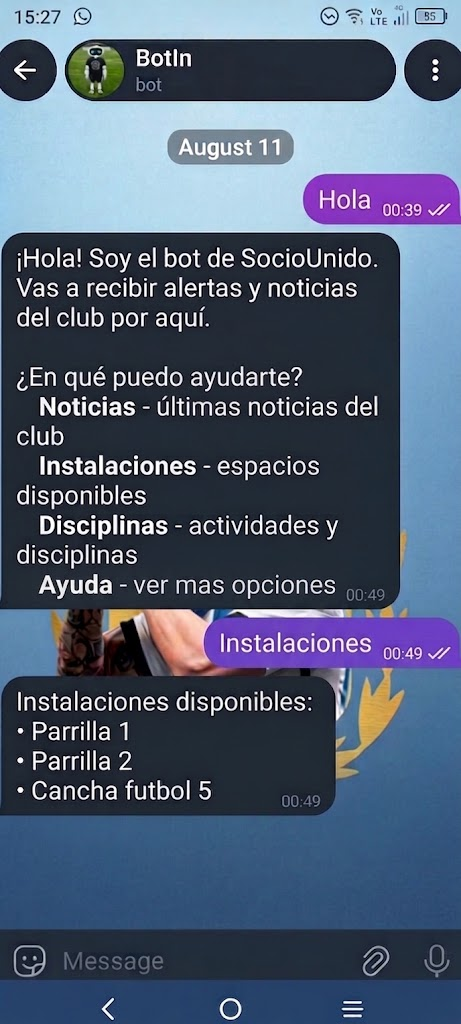
\includegraphics[width=\textwidth]{img/bot/chat.jpg}
    \end{minipage}
    \caption{Vistas del perfil verificado y ejemplo de flujo de mensajes automatizados vía Telegram.}
    \label{fig:bot_conversacional}
\end{figure}
